%\chapter{Surface Flow}
\label{sec:Surface}
%

This chapter deals with surface runoff which is flow over the land surface generated by precipitation, melting of snow, or other sources.
%
Typically, not all precipitation or snow produces runoff because storage from soil and plant roots can absorb substantial amounts of water.
%
Infiltration excess (\cite{Horton:40}) overland flow occurs when precipitation exceeds the rate at which water infiltrates into the soil (Test case \ref{sec:horton}).
%
When the soil is saturated and depression storage filled, the precipitation, even as a light shower, immediately becomes surface runoff (Borden test case).
%
Similarly, urbanization leads to more pronounced flow maxima during storm events, when impervious surfaces such as pavement force the runoff directly to the stream (Test case \ref{sec:Vcatch}).
%Accordingly, groundwater recharge is reduced which leads to a lower water table.  

Horizontal flow over a flat or moderately flat surface is described by the Saint-Venant Shallow Water Equations which read
%
\begin{eqnarray}
\phi_o\frac{\partial H}{\partial t} + \nabla H \mathbf v &= & q \label{eqn:Saint_Venant}\\
\frac{\partial \mathbf v}{\partial t} + \mathbf v \cdot \nabla \mathbf v  + g  \nabla h &= & g (S_0 - S_f)
\nonumber
\end{eqnarray}
%
where $H$, surface water depth, and $\mathbf v$, flow velocity, are primary variables, $g= 9.81$ m/s$^2$ is the gravitational acceleration, 
$h = H + b$ the surface water height, $b$ the bottom height, $S_0 = - \nabla b$ the surface slope, $S_f$ the friction slope, $q$ represents external sources / sinks, 
and $0 \leq \phi_o \leq 1$ is the surface porosity to incorporate depression storage. 
%
Equations (\ref{eqn:Saint_Venant}) can be derived from the
Reynolds averaged Navier Stokes Equations by integrating over water depth $H$ and assumption hydrostatic pressure $p= \rho g (h - z)$, where $\rho$ is the water bulk density (e.g. \cite{FerSal:04}).
The result is a depth-averaged flow field $v(x,y)$, where dispersion caused by this averaging, turbulence and surface friction effects are finally incorporated
in empiric resistance to flow relationships, i.e. the velocity $v$ is a power function of the water depth $H$. 
The general form of a resistance to flow relationship for 1D flow in an irregular channel (which involves an additional averaging over the channel breadth) is given by
%
\begin{eqnarray}
v = CS_f^j R_H^m \label{eqn:resistance}
\end{eqnarray}
%
where $j$, $m$ are parameters, $v(l)$ is the flow velocity in the channel course $l$, $R_H(l) = A /P$ the hydraulic radius of the channel, $A(l)$ its cross-section, and $P(l)$ the wetted perimeter. Remark that $R_H = H$ for 2D overland flow and $j = 1/2$, $m= 2/3$ result in the relationship by Manning where $n=1/C$ is a surface roughness parameter.
%
Neglect of the inertial terms simplifies Equations (\ref{eqn:Saint_Venant}) to the diffusive wave shallow water equation, which reads
%
\begin{eqnarray}
\phi_o\frac{\partial H}{\partial t}
- \nabla\cdot  \frac{C H R_H^m}{|\nabla h|^{1-j}}\nabla h
= q
\label{eqn:DiffusiveWave}
\end{eqnarray}
%
Further neglect of the hydrostatic pressure term in Equation (\ref{eqn:Saint_Venant2}) leads to the kinematic wave equation reading
%
\begin{eqnarray}
\phi_o\frac{\partial H}{\partial t}
+ C (m+1) R_H^m \nabla H
= q
\label{eqn:KinematicWave}
\end{eqnarray}
%
Equations (\ref{eqn:Saint_Venant})-(\ref{eqn:KinematicWave}) allow to simulate small-amplitude waves (surface runoff, flood waves).
The diffusive wave approximation (\ref{eqn:DiffusiveWave}) can capture backwater phenomena and the
Saint-Venant Equations (\ref{eqn:Saint_Venant}), further, dam break waves. 
Conditions for the applicability of the Saint-Venant approximations (kinematic and diffusive wave) 
are stated for instance in \cite{GovEtAl:88} (Test case \ref{sec:Govindaraju}), while shallow water equations to reproduce large-amplitude waves (e.g. ocean waves)
can be found in \cite{Miglio:00}.
%

%
External forcing (precipitation, infiltration, outflow, etc.) can be incorporated in the surface flow Equations (\ref{eqn:Saint_Venant})-(\ref{eqn:KinematicWave})
with source /sink terms $q$.
A normal depth $q_{\mbox{\scriptsize norm}}$ sink term assumes that water flows under uniform (normal) conditions at a downstream boundary 
while a critical depth $q_{\mbox{\scriptsize crit}}$ sink term represents free outfall:
%
\begin{eqnarray}
q_{\mbox\tiny norm} &=&- CS_o^j H^m \label{eqn:normalDepth}\\
q_{\mbox\tiny crit} &=&- \sqrt{ gH^3} \label{eqn:criticalDepth}
\end{eqnarray}
%
A \cite{Green:11} term $q_{\mbox{\tiny GA}}$ provides an effective precipitation rate
$q_{\mbox{\scriptsize prec}}^{\mbox{\scriptsize eff}} = q_{\mbox{\scriptsize prec}} - q_{\mbox{\tiny GA}}$ for overland flow on an infiltrating surface.
Since water infiltrates into dry soil as a sharp wetting front, the Green and Ampt infiltration model assumes that 
soil saturation above and below the wetting front and the soil-water suction immediately below the wetting front remain constant. 
The infiltration source term $q_{{\mbox{\tiny GA}}}(t)$ and the depth of the wetting front $a'(t)$ read
%
\begin{eqnarray}
q_{\mbox{\tiny  GA}} &=& K' \left( \frac{H - \Psi}{a'} \right) \label{eqn:OLF_Green_Ampt}\\
a' &=& \frac{\int_{0}^{t}q_{\mbox{\tiny GA}}(s)\, ds}{\Delta \Theta} .\nonumber
\end{eqnarray}
%
where $\Psi$ the effective capillary drive,  $K'$ is related to the saturated soil hydraulic conductivity in chapter Richards flow, 
and $\Delta \Theta$ the initial moisture deficit. 

%
%-------BENCHMARKS--------------------------------------------------------------------------------------------------------------
%
%

%
%
\section{One-dimensional surface flow}
\label{sec:Govindaraju}
%
\subsection{Definition}
%
\cite{Gov:88} compared surface runoff predictions with the Saint-Venant Equations (\ref{eqn:Saint_Venant}), the diffusive wave approximation (\ref{eqn:DiffusiveWave}), and 
the kinematic wave approximation (\ref{eqn:KinematicWave}) at an inclined plane.
In the selected test case (Table \ref{tab-govin} for surface roughness) the plane length is $L = 100$ m, the slope $S_0 = 0.01$, the precipitation rate $4 \cdot 10^{-3}$ m/s which results in a
kinematic wave number of $k = S_0 L / H Fr^2 =10$ and Froude number of $Fr = v / \sqrt{gH}= 0.5$. 
A normal depth boundary condition (\ref{eqn:normalDepth}) is assigned at the outlet.
The simulation time is $4$ min, time step length $1$ s, and grid size $1$ m.
%
\begin{table}[!htbp]
\caption{\label{tab-govin}Material properties.}
\begin{center}
\begin{tabular}{llrr}
\toprule
Symbol & Parameter & Value & Unit \\
\midrule
$n$ & Manning friction	  & $\unit[0.0548]{}$   & s/m$^{1/3}$ \\
\bottomrule
\end{tabular}
\end{center}
\end{table}

%
\subsection{Solution}
%
Figure \ref{OLF:giammarco} compares the surface runoff at the normal depth outet of different surface runoff simulators. The kinematic wave solution is analytically obtained.
The results of the Saint-Venant and diffusive waver solvers match well while the kinematic wave equation results in a faster rise of the hydrograph. 
%
\begin{figure} [htb!]
 \centering
 \includegraphics[width=0.75\columnwidth] {PART_II/H_SFC/govin.eps}
 \caption{Outflow comparison for one-dimensional surface runoff test case.}
 \label{OLF:govin_outlet}
\end{figure}
%
%--------------------------------------------------------------------------------------------------------------------------
%
%
\section{Surface flow on a tilted V-catchment}
\label{sec:Vcatch}
%
\subsection{Definition}
%
In the synthetic test case by \cite{Gian:96} precipitation with a rate of $3 \cdot 10^{-6}$ m/s 
is applied for $90$ min on an impervious V-catchment followed by a recession period of additional $90$ min.
The V-catchment consists of two sloping planes $800$ m wide and $1000$ m long joined by $20$ m wide and $1000$ m long channel.
At the catchment base (channel region) the surface roughness was reduced (Table \ref{tab-V-catch}) and the slope set at 
$S_0 = 0.02$. The hillslopes additionally have a slope of $S_0 = 0.05$ towards the channel. 
At the channel outlet the water leaves free-falling (critical depth sink term (\ref{eqn:criticalDepth})) 
while at the remaining boundaries no-flow is imposed.
A structured (rectangular) grid ($100$ m $\times$ $100$m) a time-step maximum length of $1$ min are selected.
%
\begin{table}[!htbp]
\caption{\label{tab-V-catch}Material properties.}
\begin{center}
\begin{tabular}{llrr}
\toprule
Symbol & Parameter & Value & Unit \\
\midrule
$n$ & Manning friction (Hillslope)	  & $\unit[0.015]{}$   & s/m$^{1/3}$ \\
$n$ & Manning friction (Channel)	  & $\unit[0.15]{}$   & s/m$^{1/3}$ \\
\bottomrule
\end{tabular}
\end{center}
\end{table}
%
\subsection{Solution}
%
Figure \ref{OLF:giammarco} compares critical depth outflow of different surface runoff simulators.
The simulated hydrographs reach a maximum roughly after $60$ min 
and the entire water has almost left the catchment after the simulation time of $180$ min.
%
\begin{figure} [htb!]
 \centering
 \includegraphics[width=0.75\columnwidth] {PART_II/H_SFC/gian.eps}
 \caption{Runoff at channel outlet for tilted V-catchment test case.}
 \label{OLF:giammarco}
\end{figure}
%--------------------------------------------------------------------------------------------------------------------------
%
\section{Infiltration excess (Horton) overland flow} \label{sec:horton}
%
\subsection{Definition}
%
In the classic experiments by \cite{Smith:71} a light oil  
was applied with a constant rate of $q_{\mbox{\scriptsize prec}} =6.944\times 10^{-5}$ m/s for $15$ min  
on an initially drained soil flume with a length of $12.2$ m, a width of $0.051$ m and a uniform slope of $0.01$.
Measured outflow at the lower flume end is compared with 1D surface runoff simulations for a grid size of $12.2$ cm and a constant time step length of $1$ s.
Parameters are stated in Table \ref{tab-horton} for flow resistance (\ref{eqn:resistance}) and a Green Ampt source term (\ref{eqn:OLF_Green_Ampt}) 
(cmp. with chapter Surface-subsurface flow coupling).
A critical depth sink term (\ref{eqn:criticalDepth}) is assigned at the flume outlet.
%
\begin{table}[!htbp]
\caption{\label{tab-horton}Material properties.}
\begin{center}
\begin{tabular}{llrr}
\toprule
Symbol          & Parameter                 & Value                      & Unit \\
\midrule
$n$             & Manning friction 	        & $\unit[0.15]$              & s/m$^{1/3}$ \\
$K$             & Conductivity 	            & $\unit[2.3\times 10^{-5}]$ & $m/s$ \\
$\Psi$          & Effective capillary drive & $\unit[0.13]$              & $m$ \\
$\Delta \Theta$ & Initial moisture deficit  & $\unit[0.3]{}$             & $-$ \\
\bottomrule
\end{tabular}
\end{center}
\end{table}
%
\subsection{Solution}
%
Fig.~\ref{SFC:resultsWool} compares measured surface runoff with model predictions at the flume outlet.
First, precipitation completely infiltrates (stage I).
After about $7$ min surface runoff starts and produces a fast rising hydrograph (stage II).
As soon as precipitation from the entire flume surface has reached the outlet, the hydrograph turns flat.  
Infiltration rate continues declining as the soil becomes saturated such that surface runoff still increases in the later part of the experiment (stage III).
The experimental hydrograph exhibits a considerable dip during stage III which is attributed to gas phase movement (\cite{Smith:71}). 
%
\begin{figure} [htb!]
 \centering
 \includegraphics[width=0.75\columnwidth] {PART_II/H_SFC/Wool.eps}
 \caption{Comparison of measured and simulated Horton overland flow.}
 \label{SFC:resultsWool}
\end{figure}
%


